%%
% TUM Corporate Design LaTeX Templates
% Based on the templates from https://www.tum.de/cd
%
% Feel free to join development on
% https://gitlab.lrz.de/tum-templates/templates
% and/or to create an issue in case of trouble.
%
% tum-article class for scientific articles, reports, exercise sheets, ...
%
%%

\documentclass[twocolumn]{tum-article}

\usepackage{booktabs}
\usepackage{enumitem}
\usepackage{lipsum}

\pgfplotsset{width=9cm,compat=1.15}
\usepackage{tum-base}
\usepackage{packages/pgf-pie/pgf-pie}
\usepackage{subcaption}
\usepackage[labelformat=parens,labelsep=quad,skip=3pt]{caption}
\usepackage{graphicx}
\usepackage{amsmath}
\usepackage{algorithm}
\usepackage[noend]{algpseudocode}
\usepackage{xspace}

\usepackage{pgfplots}
\pgfplotsset{
    barplot/.style={
        ybar,
        ymin=0,
        ymax=100,
        height=4cm,
        enlargelimits=0.15,
        ymajorgrids,
        ytick={0,25,50,75,100},
        xtick=data,
        xticklabel style={font=\scriptsize\tt},
        legend style={at={(0.5,-0.3)}, anchor=north,legend columns=-1},
    },
    barplot_mono/.style={
        barplot,
        symbolic x coords={milnet, empty, swn, vader, nltk, svm},
        xticklabels={MilNet, SWN, VADER, NLTK, SVM}
    },    
    barplot_en/.style={
        barplot,
        symbolic x coords={bert, roberta, xling, empty, nltk, svm},
        xticklabels={BERT, RoBERTa, XLING, NLTK, SVM}
    },
    barplot_de/.style={
        barplot,
        symbolic x coords={bert, roberta, xling, empty, textblob},
        xticklabels={BERT, RoBERTa, XLING, TextBlob}
    },
    barplot_en_en/.style={
        barplot_en,
        title=\taskEN,
    },
    barplot_en_org/.style={
        barplot_en,
        title=\taskORG,
    },
    barplot_en_de/.style={
        barplot_de,
        title=\taskDE,
    }
}
\newcommand{\scorelegend}{\legend{F1-micro, F1-macro}}

\newcommand{\dataORG}{{\bf organic}\xspace}
\newcommand{\dataEN}{{\bf amazon~EN}\xspace}
\newcommand{\dataDE}{{\bf amazon~DE}\xspace}
\newcommand{\taskORGORG}{{\tt organic-organic}\xspace}
\newcommand{\taskORG}{{\tt amazon~EN-organic}\xspace}
\newcommand{\taskEN}{{\tt amazon~EN-amazon~EN}\xspace}
\newcommand{\taskDE}{{\tt amazon~EN-amazon~DE}\xspace}


\title{Sentiment Analysis Using BERT and Multi-Instance Learning}
\author{Burak Iryna\authormark{1},
  Restrepo Pablo\authormark{2}}

\email{iryna.burak@tum.de, pablo.restrepo@tum.de}

\affil[1]{Department of Mathematics, Technical University of Munich (TUM),
  Boltzmannstr. 3, 85748 Garching, Germany}
\affil[2]{Department of Informatics, Technical University of Munich (TUM),
  Boltzmannstr. 3, 85748 Garching, Germany}

\date{31 July 2020}

\begin{document}

\maketitle

\begin{abstract}
  We consider the task of sentence-level sentiment analysis for data coming from the organic reviews domain. In this project, we used Multi-Instance Learning Networks combined with various initial sentence embeddings to explore both monolingual and cross-lingual settings. Additionally, we conducted experiments on a simplified task by dropping the neutral class.
\end{abstract}

\section{Introduction}
\begin{figure}[b]
\centerline{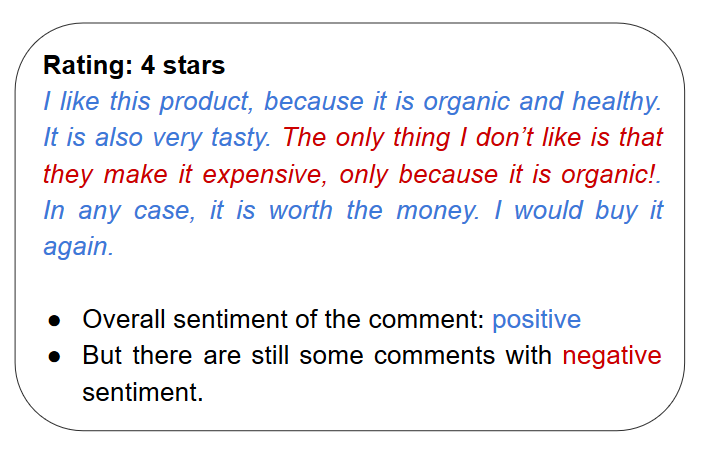
\includegraphics[scale=.5]{images/comment_example.png}}
\caption{Example of a positive comment with negative sentences.}
\label{comment_example}
\end{figure}

Today, the  long-term  goal  of  developing  sustainable  food systems is considered a high priority by several intergovernmental  organizations \cite{Mie2017}. This has lead to developments in modern organic food production, largely driven by the ideal of sustainability and environmental concern \cite{healthyNutritiousFood}.\\
In order to create successful strategies to promote production and consumption of organic food, it is necessary to understand the opinions of the general public regarding organic products. For this, it is useful to understand the sentiment of comments about organic food in a sentence level. This is illustrated in Figure \ref{comment_example} showing that even though the overall sentiment of the comment is positive, there are sentences that are clearly negative. This would be ignored if we analyzed only the sentiment of the comment, and not the sentiment of each sentence.\\
In addition to the above, Web 2.0 has led to the emergence of blogs, forums, and online social networks that enable users to discuss any topic and share their opinions about it \cite{Dang_2020}. For this reason, coarse-grained document-level annotations are relatively easy to obtain. Despite this, the acquisition of  sentence-  or  phrase-level  sentiment  labels  remains  a  laborious  and  expensive endeavor even tough they are relevant to various opinion mining applications \cite{angelidis2017multiple}, including sentiment analysis.\\
For all these reasons, a model that allows us to understand sentiment in a sentence level for the organic food domain based on comments is important.\\
In this paper, we will explore the use of Multi-Instance Learning Networks, which only require document-level supervision and learns to introspectively judge the sentiment  of  constituent  segments \cite{angelidis2017multiple} for sentence-level sentiment analysis in the context of organic food. For this, we will use use data from Amazon reviews in English and German, together with a dataset that contains annotated sentences from Quora about organic products.\\
Also, we will explore the effects of using transfer learning together with Multi-Instance Learning Networks and compare the results obtained by using different initial sentence embeddings.\\
Finally, we will investigate the use of Multi-Instance Learning Networks in cross-lingual tasks for English and German data. \\
% by analyzing the results given by models trained with data in English, when they are tested with data in German.\\


\section{Theory}
\subsection{MilNet architecture}
Multi-Instance Learning Networks were introduced in \cite{angelidis2017multiple} as a tool for predicting segment sentiment labels when having only document sentiment labels as a ground truth. In our setting, sentences are treated as segments, and comments --- as documents. \\
The process of training a MilNet can be described with the following steps (see Figure \ref{milnet}):
\begin{enumerate}[label=(\alph*)]
    \item Split each document in the dataset into segments;
    \item Compute segment embeddings as a convolution of corresponding word embeddings;
    \item Compute segment labels using a recurrent neural network with gated recurrent units;
    \item Compute document label using attention mechanism;
    \item Do backpropagation with respect to ground truth of {\bf document} labels only.
\end{enumerate}

\begin{figure}[h]
\centerline{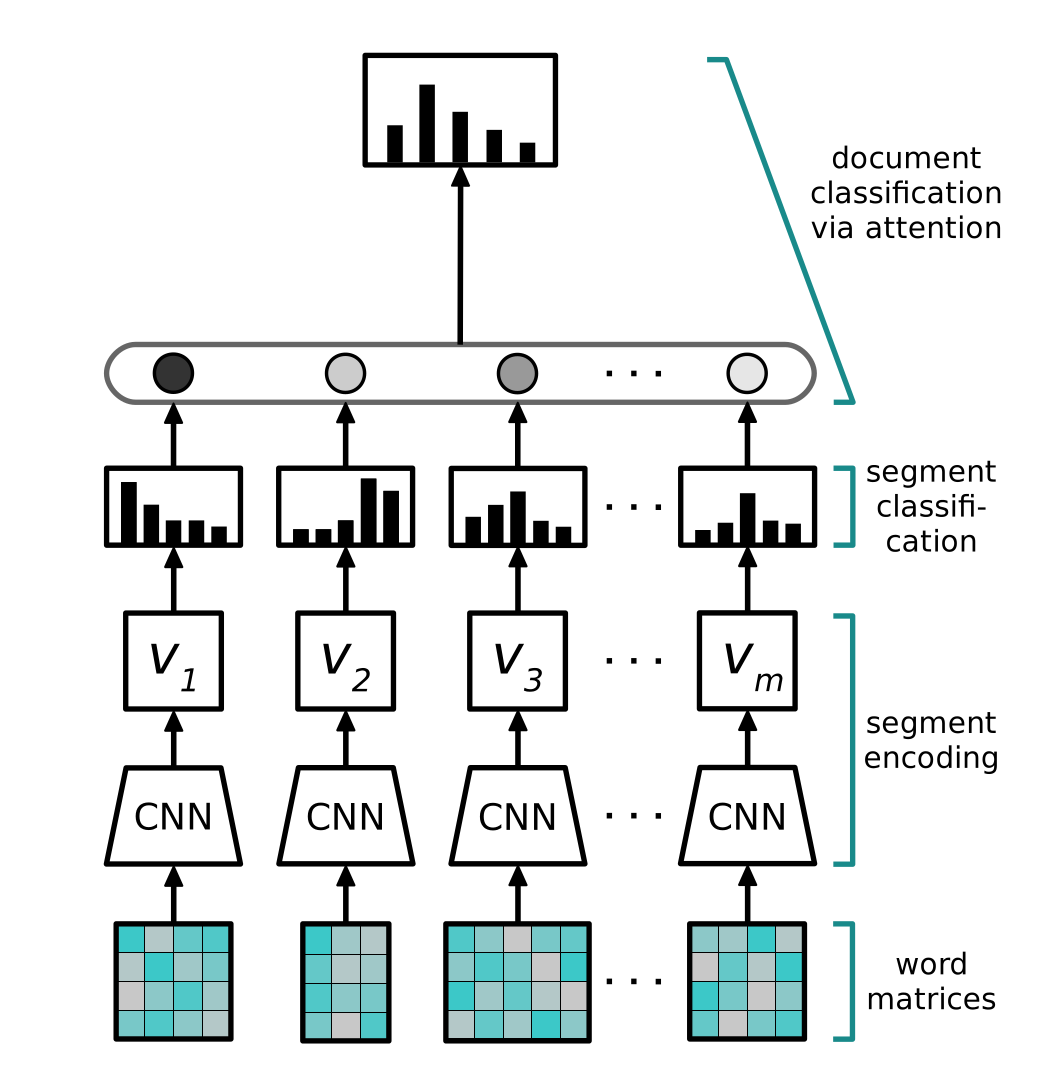
\includegraphics[scale=.2]{images/milnet.png}}
\caption{MilNet architecture.}
\label{milnet}
\end{figure}
After the training, one can extract segment sentiments by ignoring the last two steps. \\
For this project, we were interested in exploring the potential of BERT embeddings in such architecture. For this, we skipped the first two steps by using precomputed segment embeddings. 

\subsection{Embeddings}

\subsubsection{Vector semantics embeddings}
Words that occur in similar contexts tend to have similar meanings. The concept of vector semantics instantiates this linguistic hypothesis by learning representations of the meaning of words, called {\bf embeddings}, directly from their distributions in texts. These representations are used in every natural language processing application that makes use of meaning \cite{jurafskyBook}.

\subsubsection{Feature representation for neural networks}
We can think of a feed-forward neural network as a function $NN(x)$ that takes as input a $d_{in}$ dimensional vector $x$ and produces a $d_{out}$ dimensional output vector. When dealing with natural language, the input $x$ encodes features  such  as  words, part-of-speech tags or other linguistic information. Perhaps the biggest conceptual jump when moving from sparse-input linear models to neural-network based models is to stop representing each feature as a unique dimension (the so called one-hot representation) and representing them instead as dense vectors called {\bf embeddings}. That is, each core feature is embedded into a $d$ dimensional space, and represented as a vector in that space \cite{goldberg2015primer}.

\subsubsection{Contextualized Embeddings}
With traditional embeddings such as {\bf GloVe} and {\bf Word2Vec}, each word in a vocabulary gets its own representation, independent of the context on which they are used. Even though this may be useful for many problems, it is logical to think that the semantic information of a word depends on the context in which it is used. For example, consider the word "jaguar", which can have different word senses depending on the context: an animal, a car or a guitar.\\
%An example of this is the word "jaguar", which can have different word senses depending on the context: an animal, a car or a guitar.\\
Even when using the same word sense of a word, there may be semantic differences dependent on the context in which the word is used. Contextual embeddings like {\bf ELMo} and {\bf BERT} address this issue by giving each token of a sentence its own embedding depending on the entire context of the sentence.

\subsubsection{Sentence Embeddings}
Sentence embeddings are dense vectors that summarize different properties of a sentence (e.g. its meaning), thereby extending the very popular concept of word embeddings. In contrast to task-specific representations, such as the ones trained specifically for tasks like textual entailment or sentiment, such sentence embeddings are trained in a task-agnostic manner on large datasets. As a consequence, they often perform better when little labeled data is available \cite{rckl2018concatenated}.

\subsubsection{Transfer learning and model pretraining}
Language  model  pretraining  has  been  shown  to be effective for improving many natural language processing tasks \cite{devlin2018bert}. This model pretraining consists in training a neural network in one task (usually language modeling), and then using the intermediate representation of a deep layer of the network as embeddings for another model. Such approach allows to transfer the syntactic and semantic properties learned by the language modeling model to other models that focus on different tasks.\\
There  are  two  existing  strategies  for  applying pretrained language representations to downstream tasks: feature-based and fine-tuning. The feature-based  approach, such as {\bf ELMo}, uses task-specific architectures that include the pretrained representations as additional features. The fine-tuning approach, such as the Generative pretrained Transformer ({\bf OpenAIGPT}), introduces minimal task-specific  parameters,  and  is  trained  on  the downstream  tasks  by  simply  fine-tuning all pretrained parameters.

\subsubsection{BERT: Bidirectional Encoder Representations from Transformers}
{\bf BERT} improves the fine-tuning based approaches by using a “masked language  model” (MLM)  pretraining  objective. The masked language model randomly masks some of the tokens from the input, and the objective is to predict the original vocabulary id of the masked word  based only on its context \cite{devlin2018bert}.

\subsubsection{RoBERTa}
RoBERTa is an improved recipe for training BERT models, that can match or exceed the performance of all of the post-BERT methods. It includes modifications to BERT such as: (1) training the model longer, with bigger batches, over more data; (2) removing the next sentence prediction objective; (3) training on longer sequences; and (4) dynamically changing the masking pattern applied to the training data \cite{liu2019roberta}.

\subsubsection{XLING}
XLING generalizes  the  concept  of  average  word  embeddings to power mean word embeddings. In this method, instead of using the component-wise arithmetic averages of the word embeddings to generate sentence embeddings, the concateniation of the so-called power means is used \cite{rckl2018concatenated}.


\section{Experimental Setup}
\subsection{Data}
\label{data_section}
For our experiments, we used three datasets. We will be referring to them as: \dataEN, \dataORG, and \dataDE.
\subsubsection{Amazon EN}
This dataset contains Amazon product reviews and metadata from May 1996 to July 2014. In our case, since we were interested in the organic food domain, we used data from three categories:
\begin{itemize}
  \item Grocery and Gourmet Food
  \item Health and Personal Care
  \item Beauty
\end{itemize}
These three categories contained the following amount of reviews:
\begin{center}
 \begin{tabular}{||c c||} 
 \hline
 Category & Reviews\\ [0.4ex] 
 \hline\hline
 Grocery and Gourmet Food & 198.502\\ 
 \hline
 Health and Personal Care & 151.254\\
 \hline
 Beauty & 346.355\\
 \hline\hline
 Total & 696.111\\
 \hline
\end{tabular}
\end{center}
% As we are interested in the domain of organic food, we filtered all reviews that contained the word "organic". After doing this, we ended up with the following amount of reviews in each category:
Additionally, we filtered all reviews that contained the word "organic". In the end, we ended up with the following amount of reviews in each category:
\begin{center}
 \begin{tabular}{||c c||} 
 \hline
 Category & Reviews\\ [0.4ex] 
 \hline\hline
 Grocery and Gourmet Food & 9.962\\ 
 \hline
 Health and Personal Care & 3.272\\
 \hline
 Beauty & 2.227\\
 \hline\hline
 Total & 15.561 \\
 \hline
\end{tabular}
\end{center}
The percentage distribution of ratings in the dataset is shown in Figure \ref{amazon_en_pie_chart}.\\

\begin{figure}[h]
\centering
\begin{tikzpicture}
    \pie[color={TUMBlau!10, TUMBlau!25, TUMBlau!40, TUMBlau!55, TUMBlau!70},
        radius=1.5,
        text=pin,
        before number=\pgfsetfillopacity{0.0}]
        {4.34/1 (4.34\%), 4.52/2 (4.52\%), 9.87/3 (9.87\%), 19.75/4 (19.75\%), 61.49/5 (61.49\%)}
\end{tikzpicture}
\caption{Percentage distribution of ratings in \dataEN.}
\label{amazon_en_pie_chart}
\end{figure}
We can observe that the dataset is imbalanced. For this reason, we applied a downsampling strategy to balance it for our experiments.\\
To train the MilNets for our experiments, we were interested in getting the individual sentences of each comment. To split the Amazon comments into sentences, we used NLTK, which is a a suite of program modules, covering symbolic and statistical natural language processing \cite{NLTKarticle}.\\
After splitting our comments into sentences, we ended up with {\bf 129.867} sentences. Figure \ref{sentences_per_comment_amazon_en} shows the number of sentences per comment in the dataset.
\begin{figure}[h]
\centerline{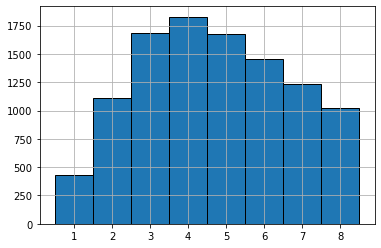
\includegraphics[scale=.4]{images/sentences_per_comment_amazon_en.png}}
\caption{Number of sentences per comment in \dataEN.}
\label{sentences_per_comment_amazon_en}
\end{figure}\\
In this histogram we can see that most of the comments contain between 3 and 5 sentences, which shows that the dataset is appropriate for our MilNet Experiments.\\
In many of our experiments, we used {\bf BERT} to generate embeddings for our sentences. As {\bf BERT} can only handle sentences with a maximum of 512 tokens including [CLS] and [SEP], we removed the outlier sentences that had a large number of tokens. For \dataEN, only 0.2\% of the sentences contain more than 100 tokens. For this reason, we removed all sentences that surpassed that limit.\\
%Figure \ref{amazon_en_tokens_per_sentence} shows the number of tokens per sentence of the dataset after removing the outlier sentences with more than 100 tokens. In this figure we can see that most of the sentences have around 20 tokens.
Figure \ref{amazon_en_tokens_per_sentence} shows the number of tokens per sentence of the dataset after removing the outlier sentences. In this figure we can see that most of the sentences have around 20 tokens.
\begin{figure}[h]
\centerline{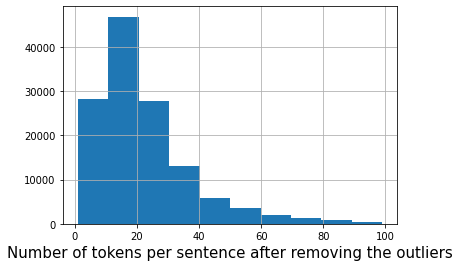
\includegraphics[scale=.5]{images/tokens_per_sentence_amazon_eng_after.png}}
\caption{Number of tokens per sentence in \dataEN.}
\label{amazon_en_tokens_per_sentence}
\end{figure}
\subsubsection{Organic}
This dataset contains sentences with opinions about organic products from Quora. The sentiment of this sentences has been annotated by domain experts with the categories: positive, negative and neutral. The dataset is divided in train, validation and test data.\\
After removing all the 'nan' values, we ended up with the following amount of sentences, with the following distributions:
\begin{center}
 \begin{tabular}{||c c c||} 
 \multicolumn{3}{c}{\bf Train dataset} \\
 \hline
 Sentiment & Sentences & \%\\ [0.4ex] 
 \hline\hline
 positive & 1500 & 32\%\\ 
 \hline
 negative & 1375 & 29.33\%\\
 \hline
 neutral & 1812 & 38.66\\
 \hline\hline
 Total & 4687 & \\
 \hline
\end{tabular}
\end{center}
We can observe that the data is only slightly unbalanced. Therefore, no balancing strategy was applied to this dataset for our experiments.\\
In this dataset, less than 1\% of the data has more than 100 tokens. For this reason, we removed those outliers, just as we did with \dataEN. Figure \ref{organic_tokens_per_sentence} shows the number of tokens per sentence of the dataset after removing the outlier sentences. In this figure we can observe that the final distribution is similar to the one for \dataEN.\\
\begin{figure}[h]
\centerline{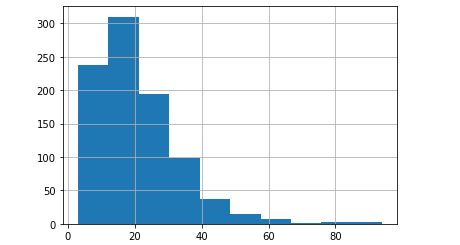
\includegraphics[scale=.5]{images/tokens_per_sentence_organic_after.png}}
\caption{Number of tokens per sentence {\bf Organic}}
\label{organic_tokens_per_sentence}
\end{figure}\\
\subsubsection{Amazon DE}
This dataset contains Amazon reviews in the German language. Since our domain is organic products, we used the data from the two categories:
\begin{itemize}
  \item Grocery
  \item Beauty
\end{itemize}
The dataset contains the following amount of reviews in the selected categories:\\
\begin{center}
 \begin{tabular}{||c c||} 
 \hline
 Category & Reviews\\ [0.4ex] 
 \hline\hline
 Grocery & 2737\\ 
 \hline
 Beauty & 7162\\
 \hline
\end{tabular}
\end{center}
The percentage distribution of ratings in the dataset is shown in Figure \ref{amazon_de_pie_chart}.\\
\begin{figure}[h]
\centering
\begin{tikzpicture}
    \pie[color={TUMBlau!10, TUMBlau!25, TUMBlau!40, TUMBlau!55, TUMBlau!70},
        radius=1.5,
        text=pin,
        before number=\pgfsetfillopacity{0.0}]
        {21.20/1 (21.20\%), 20.63/2 (20.63\%), 20.54/3 (20.54\%),
        18.08/4 (18.08\%), 19.52/5 (19.52\%)}
\end{tikzpicture}
\caption{Percentage distribution of ratings in {\bf amazon DE} dataset.}
\label{amazon_de_pie_chart}
\end{figure}\\
We can observe that the dataset is balanced. For this reason, no balancing strategy was applied to it in our experiments.\\
Just as we did with \dataEN, we used NLTK to split this dataset into sentences. After doing so, we ended up with {\bf 28.994} sentences. Figure \ref{sentences_per_comment_amazon_de} shows the number of sentences per comment in the dataset.\\
\begin{figure}[h]
\centerline{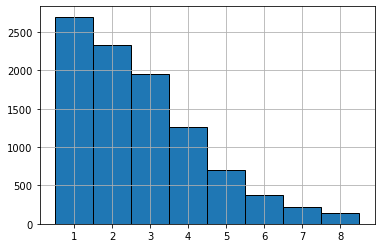
\includegraphics[scale=.5]{images/sentences_per_comment_amazon_de.png}}
\caption{Number of sentences per comment in \dataDE.}
\label{sentences_per_comment_amazon_de}
\end{figure}
After filtering the relevant categories, only 3 sentences in the dataset had more than 100 tokens. We removed these outliers for our experiments. Figure \ref{amazon_de_tokens_per_sentence} shows the number of tokens per sentence after removing the outliers.\\
\begin{figure}[h]
\centerline{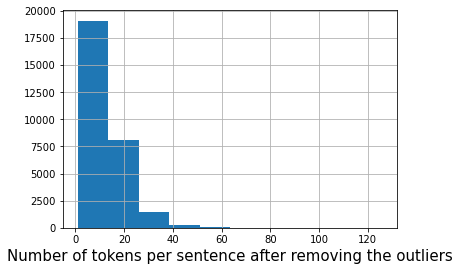
\includegraphics[scale=.5]{images/tokens_per_sentence_amazon_de_after.png}}
\caption{Number of sentences per comment in \dataDE.}
\label{amazon_de_tokens_per_sentence}
\end{figure}
It is interesting to see how different the distributions for \dataDE shown in figure \ref{sentences_per_comment_amazon_de} and figure \ref{amazon_de_tokens_per_sentence} are from those shown in figure \ref{sentences_per_comment_amazon_en} and \ref{amazon_en_tokens_per_sentence} for \dataEN. When comparing these distributions, it can be concluded that German authors tend to write comments with fewer sentences than English ones, but those sentences are longer.
\subsection{Sentiment assessment from review ratings}
In our case, we are interested in using our data to predict sentiment.\\
Given that most of our data consists of Amazon reviews with the number of stars given by the customer, we required a strategy to asses the sentiment of a review based on its stars. The strategy that we used for this purpose is described in Algorithm \ref{sentiment_assesment_algorithm}.\\
\begin{algorithm}[b]
\caption{Sentiment Assessment from number of stars}\label{euclid}
\label{sentiment_assesment_algorithm}
\begin{algorithmic}[1]
\Procedure{SentimentAssessment}{}
\If {$\textit{numberOfStars} < 3$}
    \State $\textit{sentiment} \gets \text{negative}$
\ElsIf {$\textit{numberOfStars} = 3$}
    \State $\textit{sentiment} \gets \text{neutral}$
\Else
    \State $\textit{sentiment} \gets \text{positive}$
\EndIf
\Return \textit{sentiment}
\EndProcedure
\end{algorithmic}
\end{algorithm}
Figure \ref{amazon_sentiment_pie_chart} shows the distribution of sentiment for these datasets after splitting them into sentences and extracting sentiment from them using the described strategy.\\
\begin{figure}[h]
{\bf Amazon EN}:\\
\begin{tikzpicture}
    \pie[color={TUMBlau!10, TUMBlau!40, TUMBlau!70},
        radius=1,
        text=pin,
        before number=\pgfsetfillopacity{0.0}]
        {78.25/positive (78.25\%), 10.63/negative (10.63\%), 11.10/neutral (11.10 \%)}
\end{tikzpicture}\\
{\bf Amazon DE}:\\
\begin{tikzpicture}
       \pie[color={TUMBlau!10, TUMBlau!40, TUMBlau!70},
        radius=1,
        text=pin,
        before number=\pgfsetfillopacity{0.0},
        rotate=90]
        {37.88/positive (37.88\%), 41.84/negative (41.84\%), 20.26/neutral (20.26\%)}
\end{tikzpicture}
\caption{Sentiment distribution for \dataEN and \dataDE after extracting sentiment from reviews}
\label{amazon_sentiment_pie_chart}
\end{figure}\\
In total we had 131.349 sentences in {\dataEN} and 28.994 in {\dataDE}.\\
\subsection{Embeddings}
In our experiments, we used different types of embeddings for our data. In this section we will describe how we got embeddings for each experiment using different models and tools.
\subsubsection{Embeddings for monolingual experiments}
For our monolingual experiments, we used BERT base uncased to generate embeddings for our sentences. For this, we used the tool "Bert as a service".\\
In order to make use of all the syntactic and semantic properties learned by BERT, it is necessary to use a deep layer of the model for the embeddings generation. Nevertheless, the last layer of the model is too close to the target functions, which means that embeddings extracted from this level may be biased towards those targets. For these reasons, we used the second-to-last layer from the BERT model to generate embeddings for the tokens of our sentences.\\
As pooling strategy to get sentence embeddings, we used the mean of the tokens of the sentence.\\
\subsubsection{Embeddings for cross-lingual experiments}
For our cross-lingual experiments, we used different models and tools:\\\\
{\bf Multilingual Bert}:\\
For the cross-lingual BERT experiments, we used the model "Bert Base Multilingual Cased" and the tool "Bert as a service". To generate embeddings for our sentences, we used the -2 layer (second-to-last) and the mean of the tokens as pooling strategy.\\\\
{\bf RoBERTa}:\\
To generate embeddings with RoBERTa, we used the RoBERTa  model provided by the transformers library. Also, we used the library sentence-transformers to generate sentence embeddings. As we did with our other BERT models, we used the -2 layer and the mean of the tokens as pooling strategy.\\\\
{\bf XLING}:\\
For the generation of XLING embeddings, we used the Tensorflow module: universal-sentence-encoder-xling-many. Also, we used the sentencepiece library as tokenizer for our sentences.
\subsubsection{Different context level embeddings}
 \label{contexLeveLEmbeddings}
For the experiment described in section \ref{sentenceCommentLevelContextExperiment}, we used BERT base uncased layer -2 and the mean of the tokens to generate sentence embeddings.
\subsection{Baselines}
In the project, we used different baselines to compare with our results.\\
In this section we are going to explain the baselines we used and the data used for training them.
\subsubsection{Sentiwordnet}
SENTIWORDNET is the result of the automatic annotation of all the synsets of WORDNET according to the notions of “positivity”, “negativity”, and “neutrality”. Each synsets is  associated  to  three numerical  scores: Pos(s), Neg(s), and Obj(s) which  indicate  how  positive, negative, and “objective” (i.e., neutral) the terms contained in the synset are \cite{sentiWordnet}. We used this tool to test sentiment in {\dataEN} and {\dataORG}.\\
Algorithm \ref{sentiwordnet_algorithm_3_classes} shows the prodedure we used to extract sentiment from our sentences using sentiwordnet. In our experiments, we used alpha = 0.3\\
\begin{algorithm}[h]
\caption{Sentiment extraction using Sentiwordnet for three classes}\label{euclid}
\label{sentiwordnet_algorithm_3_classes}
\begin{algorithmic}[1]
\Procedure{GetSentiment (\textit{sentence, alpha})}{}
\For{\textbf{each} word in sentence}
\State $\textit{word} \gets \textit{lemmatizeSentence(word)}$
\State $\textit{word} \gets \textit{getMostCommonSynset(word)}$
\State $\textit{wordSent} \gets \textit{getWordSentiment(word)}$
\State $\textit{sentenceSent} \gets \textit{sentenceSent} + \textit{wordSentPositive} - \textit{wordSentNegative}$
\EndFor
\If {$\textit{alpha} * -1 <= \textit{sentenceSent} <= \textit{alpha}$}
    \Return \textit{neutral}
\ElsIf {$\textit{sentenceSent} >= 0$}
    \Return \textit{positive}
\Else
    \Return \textit{neutral}
\EndIf
\EndProcedure
\end{algorithmic}
\end{algorithm}
For our experiments with two classes, we used the procedure shown in algorithm \ref{sentiwordnet_algorithm_2_classes}.
\begin{algorithm}[h]
\caption{Sentiment extraction using Sentiwordnet for three classes}\label{euclid}
\label{sentiwordnet_algorithm_2_classes}
\begin{algorithmic}[1]
\Procedure{GetSentiment (\textit{sentence, alpha})}{}
\For{\textbf{each} word in sentence}
\State $\textit{word} \gets \textit{lemmatizeSentence(word)}$
\State $\textit{word} \gets \textit{getMostCommonSynset(word)}$
\State $\textit{wordSent} \gets \textit{getWordSentiment(word)}$
\State $\textit{sentenceSent} \gets \textit{sentenceSent} + \textit{wordSentPositive} - \textit{wordSentNegative}$
\EndFor
\If {$\textit{sentenceSent} >= 0$}
    \Return \textit{positive}
\Else
    \Return \textit{negative}
\EndIf
\EndProcedure
\end{algorithmic}
\end{algorithm}
\subsubsection{VADER}
VADER is a simple rule-based model for general sentiment  analysis that performs  exceptionally well  in  the  social  media  domain \cite{VADERarticle}.
In our case, we used VADER to test sentiment in {\dataEN} and {\dataORG}.
\subsubsection{TextBlobDE}
TextBlob is a library for processing textual data. It provides a simple API for diving into common natural language processing tasks such as sentiment analysis \cite{textblob}. TextblobDE is an extension of this library for the German Language. We used TextBlobDE to test sentiment on {\bf Amazon DE}.
\subsubsection{NLTK sentiment analyzer}
For this baseline, we used NLTK Sentiment Analizer to train a Naive Bayes model using our data both for training and testing.
\subsubsection{Scikit-learn SVM model}
As our last baseline, we trained an SVM model using Scikit-learn. For this model, we used bigrams in order to preserve a little bit more context of the sentence for classification.
\subsection{Experiments}
\label{experimentsSection}
For all the experiments, we were using sentence embeddings as input features and comment sentiments as ground truth labels.
\subsubsection{Monolingual analysis}
We started the project with {\it monolingual} experiments --- for this setting, we worked only with data in English, i.e. {\bf amazon EN} and {\bf organic} datasets. \\
The motivation for the whole project was the idea that the {\bf amazon EN} dataset contains some useful information that can help with classifying the {\bf organic} dataset as they share the same domain. Thus, the main experiments for monolingual setting were the following:
\begin{itemize}
    \item {\tt amazon EN-organic} --- training on the {\bf amazon EN} dataset and testing on the {\bf organic} dataset.
    \item {\tt amazon EN-amazon EN} --- training and testing on the {\bf amazon EN} dataset.
\end{itemize}
For both of the experiments, we also had an option of fine-tuning the model on the {\bf organic} dataset. \\
For comparison purposes, we conducted {\tt organic-organic} experiment as well. For this, we considered each sentence in the {\bf organic} dataset as a separate comment, and fed such training data into MilNet. This led to the degenerate attention mechanism in the network as the only attention weight was equal to $1.0$ for every data point. Using this approach, we turned MulNet into a simple RNN model and obtained a competitive baseline for other experiments on the {\bf organic} dataset.

\subsubsection{Cross-lingual analysis}
The next stage of the project was introducing new dataset in German --- {\bf amazon DE}. We were interested how well the model can transfer semantic features from one language to another. Thus, we held out the whole {\bf amazon DE} dataset as a test set and conducted an experiment {\tt amazon EN-amazon DE}. \\
In the cross-lingual setting, we expored different initial embeddings, e.g. BERT multilingual, RoBerta and XLING.
\subsubsection{Different context level embeddings}
\label{sentenceCommentLevelContextExperiment}
Another area of investigation was to see if giving more context to our sentences when generating ist embeddings gave an improvement in the sentiment analysis task.
In our previous experiments, we used only the sentence as context for generating embeddings. For this experiment, we generated the embeddings of our sentences using the entire comment as context.
The following example illustrates this:\\\\
{\bf Generation of sentence-level context embeddings:}\\\\
{\bf Tokenized Comment}: CLS, {\color{TUMBlau}'I', 'really', 'love', 'the', 'product', '.'},{\color{red}'It', 'is', 'really', 'tas', '\#\#ty'}, SEP.\\
\begin{itemize}
  \item Context for the generating embeddings for {\color{TUMBlau} sentence 1}: 'I', 'really', 'love', 'the', 'product', '.'
  \item Tokens used for the generating embeddings for {\color{TUMBlau} sentence 1}: 'I', 'really', 'love', 'the', 'product', '.'
  \item Context for the generating embeddings for {\color{red} sentence 2}: 'It', 'is', 'really', 'tas', '\#\#ty'.
  \item Tokens used for the generating embeddings for {\color{red} sentence 2}: 'It', 'is', 'really', 'tas', '\#\#ty'.
\end{itemize}
{\bf Generation of comment-level context embeddings:}\\\\
{\bf Tokenized Comment}: CLS,{\color{TUMBlau}'I', 'really', 'love', 'the', 'product', '.'},{\color{red}'It', 'is', 'really', 'tas', '\#\#ty'},SEP.
\begin{itemize}
  \item Context for the generating embeddings for {\color{TUMBlau} sentence 1}: 'I', 'really', 'love', 'the', 'product', '.','It', 'is', 'really', 'tas', '\#\#ty'
  \item Tokens used for the generating embeddings for {\color{TUMBlau} sentence 1}: 'I', 'really', 'love', 'the', 'product', '.'
  \item Context for the generating embeddings for {\color{red} sentence 2}: 'I', 'really', 'love', 'the', 'product', '.','It', 'is', 'really', 'tas', '\#\#ty'.
  \item Tokens used for the generating embeddings for {\color{red} sentence 2}: 'It', 'is', 'really', 'tas', '\#\#ty'.
\end{itemize}
For getting both types of embeddings, we used BERT base uncased layer -2 and the mean of the tokens as pooling strategy to get sentences embeddings.\\
As mentioned before, BERT can only handle sentences with a maximum of 512 tokens including [CLS] and [SEP]. In our data, 9,3\% of the comments had 510 tokens or more.\\
After removing these otulier comments, we lost 34\% of our total sentences. This explains why the results in this experiment are lower compared to the other experiments we did.
\subsubsection{Two-class analysis}
The confusion matrix for the conducted experiments gave us a motivation for exploring the reduced problem with only two classes ({\it negative} and {\it positive}). As you can see in Figure \ref{confusion}, {\it neutral} class introduces a lot of confusion for the model. Thus, we dropped the {\it neutral} class from all the datasets and repeated the experiments on this reduced data.
\begin{figure}
\begin{center}
 \begin{tabular}{|c || c | c | c|} 
 \hline
 True & - & 0 & + \\
 \hline
 - & 154 & 67 & 12 \\
 0 & 70 & 174 & 44 \\
 + & 46 & 55 & 141 \\
 \hline
\end{tabular}
\end{center}
\caption{Confusion matrix for {\tt amazon EN-organic} trained on BERT base embeddings.}
\label{confusion}
\end{figure}

\section{Results}
We were using both micro and macro F1 scores as target metrics.
\subsection{Monolingual}
We trained our network on BERT base embeddings for two tasks: \taskEN and \taskORG. The main interest was to compare fine-tuned and not fine-tuned models. \\ 
\begin{figure}[h]
\begin{tikzpicture}

\begin{axis}[
    barplot,
    symbolic x coords={am_f, or_f, empty, am_nf, or_nf},
    xticklabels={amazon EN, organic, amazon EN, organic},
    ]
\addplot[fill=TUMBlau] coordinates {(am_f,45.1) (or_f,61.5) (am_nf,53.1) (or_nf,41.8)};
\addplot[fill=TUMBlauHell] coordinates {(am_f,44) (or_f,61.7) (am_nf,52.7) (or_nf,37.3)};
\scorelegend
\end{axis}

\end{tikzpicture}
\caption{Monolingual tasks {\tt amazon EN-amazon EN} and {\tt amazon EN-organic}: with fine-tuning (left) and without fine-tuning (right).}
\label{monolingual_finetune}
\end{figure}
As you can see in Figure \ref{monolingual_finetune}, training only on \dataEN yields poor results for \dataORG, while fine-tuning on \dataORG significantly drops the performance on \dataEN. Such effect may occur because comments in \dataEN and \dataORG have different structure or they've been annotated in slightly different ways. \\
Figure \ref{monolingual_finetune} shows that we should not fine-tune the model if we want to get the best results for \dataEN. Thus, from now on task \taskORG will always imply that fine-tuning on \dataORG was performed; task \taskEN -- that it was not. \\
\begin{figure}[h]

\begin{tikzpicture}

\begin{axis}[barplot_mono, name=en_en]
\addplot[fill=TUMBlau] coordinates {(milnet, 53.1) (swn, 32.9) (vader, 47.3) (nltk, 38.2) (svm, 47.4)};
\addplot[fill=TUMBlauHell] coordinates {(milnet, 52.7) (swn, 27.4) (vader, 34) (nltk, 37) (svm, 47.4)};
\end{axis}

\begin{axis}[
    barplot_mono,
    name=en_org,
    at=(en_en.below south),
    anchor=above north,
    ]
\addplot[fill=TUMBlau] coordinates {(milnet, 61.5) (swn, 38.5) (vader, 48) (nltk, 35.7) (svm, 37.8)};
\addplot[fill=TUMBlauHell] coordinates {(milnet, 61.7) (swn, 37.7) (vader, 44.3) (nltk, 18.8) (svm, 28.3)};
\end{axis}

\begin{axis}[
    barplot_mono,
    name=org_org,
    at=(en_org.below south),
    anchor=above north,
    xticklabels={MilNet, SWN, VADER, NLTK, SVM},
    ]
\addplot[fill=TUMBlau] coordinates {(milnet, 60.5) (swn, 38.5) (vader, 48) (nltk, 45) (svm, 45.7)};
\addplot[fill=TUMBlauHell] coordinates {(milnet, 60.6) (swn, 37.7) (vader, 44.3) (nltk, 43.8) (svm, 43.7)};

\scorelegend
\end{axis}

\end{tikzpicture}
\caption{Comparison of MilNet and baselines for the monolingual experiments: {\tt amazon EN-amazon EN} (top), {\tt amazon EN-organic} (middle) and {\tt organic-organic} (bottom)}.
\label{monolingual_results}
\end{figure}

In Figure \ref{monolingual_results} you can see the results for all the monolingual experiments. The plots show that task \taskORGORG is easier than \taskORG not only for our model but for the baselines as well. Again, it may be the evidence of some notable distinctions between \dataEN and \dataORG.
\subsection{Cross-lingual}
Figure \ref{crosslingual_results} shows the results for our cross-lingual experiments performed on different initial embeddings. We can see that for the first two tasks all the embeddings produced similar results. Interestingly, although \dataEN was used only as a test set, all the embeddings yielded better F1-micro scores for \taskDE than for \taskEN. Possibly, this result could be explained by the quality of \taskDE and the features of the German language --- for example, one could suggest that Germans express their opinions in a clearer way.
\begin{figure}[h]
\begin{tikzpicture}

\begin{axis}[
    barplot_en,
    name=en_en,
    ]
\addplot[fill=TUMBlau] coordinates {(bert, 48.1) (roberta, 49.3) (xling, 51.6) (nltk, 38.2) (svm, 47.4)};
\addplot[fill=TUMBlauHell] coordinates {(bert, 48.2) (roberta, 48.9) (xling, 51.2) (nltk, 37) (svm, 47.4)};
\end{axis}


\begin{axis}[
    barplot_en,
    name=en_org,
    at=(en_en.below south),
    anchor=above north,
    xticklabels={BERT, RoBERTa, XLING, NLTK, SVM},
    ]
\addplot[fill=TUMBlau] coordinates {(bert, 56.6) (roberta, 58.1) (xling, 52.1) (nltk, 35.7) (svm, 37.8)};
\addplot[fill=TUMBlauHell] coordinates {(bert, 56) (roberta, 55.7) (xling, 49.8) (nltk, 18.8) (svm, 28.3)};
\end{axis}

\begin{axis}[
    barplot_de,
    name=en_de,
    at=(en_org.below south),
    anchor=above north,
    xticklabels={BERT, RoBERTa, XLING, TextBlob},
    ]
\addplot[fill=TUMBlau] coordinates {(bert, 50.7) (roberta, 53.8) (xling, 66.4) (textblob, 37.1)};
\addplot[fill=TUMBlauHell] coordinates {(bert, 41.5) (roberta, 40.2) (xling, 59.3) (textblob, 36.6)};

\scorelegend
\end{axis}

\end{tikzpicture}
\caption{Comparison of different multilingual embeddings and baselines: {\tt amazon EN-amazon EN} (top), {\tt amazon EN-organic} (middle) and {\tt amazon~EN-amazon~DE} (bottom)}.
\label{crosslingual_results}
\end{figure}
\subsection{Different context level embeddings}
In our next experiment, we compared two models trained on BERT multilingual embeddings with different levels of context: "comment as a context"\ and "sentence as a context". As was described in section \ref{contexLeveLEmbeddings}, for getting valid embeddings we had to discard a large portion of the data. Thus, the results in the Figure \ref{crosslingual_context} for \dataEN are worse than the ones shows in the Figure \ref{crosslingual_results}. \\
Note that comment-level context coincides with sentence-level context for comments having only one sentence. For this reason, we didn't run this experiment for \dataORG. \\
As you can see in Figure \ref{crosslingual_context}, for our task comment-level context didn't cause any significant improvement in the results.
\begin{figure}[h]
\begin{tikzpicture}
\begin{axis}[
    barplot,
    symbolic x coords={en_c, de_c, empty, en_s, de_s},
    xtick=data,
    xticklabels={amazon EN, amazon DE, amazon EN, amazon DE},
    ]
\addplot[fill=TUMBlau] coordinates {(en_c,52.7) (de_c,53.1) (en_s,48.6) (de_s,52.4)};
\addplot[fill=TUMBlauHell] coordinates {(en_c,52.6) (de_c,48.9) (en_s,48.2) (de_s,50.4)};
\scorelegend
\end{axis}
	
\end{tikzpicture}

\caption{Cross-lingual {\tt amazon EN-amazon EN} and {\tt amazon EN-amazon DE}: comment-level context (left) and sentence-level context (right).}
\label{crosslingual_context}
\end{figure}
\subsection{Two-class}
As our last step, we trained a model for predicting one of the two sentiments: {\it negative} or {\tt positive}. 
\begin{figure}[h]
\begin{tikzpicture}

\begin{axis}[
    barplot_en_en,
    name=en_en,
    ]
\addplot[fill=TUMBlau] coordinates {(bert, 48.2) (roberta, 48.9) (xling, 51.2) (nltk, 37.0) (svm, 47.4)};
\addplot[fill=TUMBlauHell] coordinates {(bert, 65.1) (roberta, 71.2) (xling, 72.6) (nltk, 54.6) (svm, 65.8)};
\end{axis}

\begin{axis}[
    barplot_en_org,
    name=en_org,
    at=(en_en.below south),
    anchor=above north,
    ]
\addplot[fill=TUMBlau] coordinates {(bert, 56.0) (roberta, 55.7) (xling, 49.8) (nltk, 18.8) (svm, 28.3)};
\addplot[fill=TUMBlauHell] coordinates {(bert, 73.9) (roberta, 75.5) (xling, 83.6) (nltk, 39.5) (svm, 47.3)};
\end{axis}

\begin{axis}[
    barplot_en_de,
    name=en_de,
    at=(en_org.below south),
    anchor=above north,
    ]
\addplot[fill=TUMBlau] coordinates {(bert, 41.5) (roberta, 40.2) (xling, 59.3) (textblob, 36.6)};
\addplot[fill=TUMBlauHell] coordinates {(bert, 69.2) (roberta, 73.0) (xling, 71.5) (textblob, 49.7)};
\legend{3 classes, 2 classes}
\end{axis}

\end{tikzpicture}
\caption{Obtained F1-macro scores for the two-class task.}
\label{two_class_results}
\end{figure}
Figure \ref{two_class_results} shows that for all the experiments reducing the number of classes triggers major improvements in F1-macro score. Similarly to the Figure \ref{crosslingual_results}, for the two-class problem \taskDE produces better results than \taskEN.

\section{Conclusions}
\begin{itemize}
    \item In all of our experiments, MilNet outperformed all the baselines. This shows that it is indeed a valid technique for the sentiment analysis that can lead to good results.
    \item Even when they come from the same domain and context, {\bf Amazon EN} and {\bf Amazon DE} have notorious differences because of the language. This is reflected not only in the structure of the sentences themselves, but also in the results obtained in our classification experiments. For some experiments, results for the German data are better, possibly, due to the features of the language and the quality of the dataset.
    \item In our setting, comment-level context for embeddings didn't produce significantly better results than sentence-level context.
    \item For most of the experiments, different embedding produced similar results. In the overall result, XLING produced the best results for the task. Despite this, this result can not be generalized, because the embedding selection depends heavily on the task and data used.
    \item Presence of {\it 'neutral'} sentiment makes the task much harder for the models and baselines. This is probably because models choose to predict {\it 'neutral'} when unsure about the decision.
    \item Originally, the idea of the project was to train a model on {\bf amazon EN} and then fine-tune in on {\bf organic}. This approach gave just a small improvement on the results of pure {\bf organic} training;
    \item Neither Amazon nor organic data use the whole power of the MilNet architecture. We have only comment-level labels for the Amazon data, hence, we cannot properly test the performance on the task of predicting sentiments for individual sentences. For the organic data, the situation is opposite: we have only sentence-level labels, so we cannot properly train all the levels of the model.
\end{itemize}

\section*{Acknowledgements}
We want to thank Gerhard Hagerer, M.Sc., for a great lab course. We learned a lot from it, and we had a lot of fun!

\bibliographystyle{apalike}
\bibliography{literature}

\end{document}
